\chapter{کارهای پیشین}
\label{chapter:literature}

در این فصل به بررسی پژوهش‌های گذشته بر روی مسئله‌ی کدگذاری اندیس منعطف می‌پردازیم.

همان‌طور که در فصل اول گفته شد، مسئله‌ی کدگذاری اندیس منعطف توسط براهما و فرگولی در سال 2015 در
\cite{pliablefirstpaper}
به عنوان توسعه‌ای از مسئله‌ی کدگذاری اندیس معرفی شد. در این مسئله هر گیرنده به جای این‌که به دنبال یک پیام خاص باشد، به دنبال یک پیام جدید است که در مجموعه‌ی اطلاعات جانبی‌‌اش نباشد.

این مسئله کاربردهای مختلفی در مسائل حوزه‌های گوناگون دارد. برای مثال در محاسبات توزیع‌شده
\cite{datashuf}
\transf{سیستم‌های پیشنهاد دهنده}{recommendation system}
\cite{8404065}
\transf{یادگیری توزیع شده}{distributed learning}
\cite{8682270}.
در این فصل به مرور ادبیات پژوهشی 
\picod
می‌پردازیم.

پس از تعریف دقیق مسئله، نشان می‌دهیم که 
\picod
\nphard 
است. پس از آن الگوریتم‌های
\lr{GRCOV1}،
\lr{GRCOV2}
و
\lr{SETCOV}
را در حالت‌های تک‌ارسال و چندارسال بررسی می‌کنیم. در نهایت به بررسی الگوریتم
\lr{BinGreedy}
که یک الگوریتم قطعی تقریبی است می‌پردازیم.

در این فصل با بررسی مقالات مختلفی مثل
\cite{pliablefirstpaper,6620405, pliable2015paper,  song2017polynomialtime}
(نسخه ژرنالی مقاله دوم
\cite{pliable2016})
از فرگولی و همکاران به تعریف دقیق مسئله می‌پردازیم. فرگولی در این مقالات با تعریف مسئله برای اولین بار به مرور نتایج مختلفی را اثبات می‌کند.
\section{تعریف دقیق مسئله}
\label{sec:3:3}
	سیستمی با یک فرستنده و 
	$n$
	گیرنده در نظر بگیرید. فرستنده، مقدار
	$m$
	متغیر تصادفی
	$X = (X_1, \ldots, X_n): X_i \in \mathbb{F}$
	مشاهده‌شده را در دست دارد. هر گیرنده‌ای مانند 
	$i$،
	بخشی از متغیرهای تصادفی را در اختیار دارد که اندیس آن‌ها را با 
	$S_i \subseteq [m]$
	نشان می‌دهیم. هر گیرنده می‌خواهد 
	$t$
	پیام که جزء اطلاعات جانبی‌اش نیست یعنی اندیسشان در
	$R_i = [m] \setminus S_i$
	باشد را بازیابی کند.
	
	فرستنده می‌تواند تعدادی پیام مانند
	$Y = (Y_1, \ldots, Y_l): Y_i \in \fq$
	را برای تمام گیرنده‌ها ارسال کند تا گیرنده‌ها بتوانند با پیام‌های ارسالی و اطلاعات جانبی خود پیام‌های مورد نظر را بازیابی کنند. در
	\picod
	قبل از ارسال پیام‌ها توسط فرستنده، پیام‌هایی که توسط هر گیرنده بازیابی خواهد کرد یعنی
	$\sigma_i \subseteq R_i,  |\sigma_i| = t$
	 مشخص می‌شود. برعکس 
	\icod
	 که هر گیرنده پیامی مشخص را باید بازیابی کند در این‌جا مشخص کردن پیام‌هایی که بازیابی می‌شوند نیز بخشی از مسئله است.
	 
	 مسئله 
	 \picodt
	 پیدا کردن الگوریتمی است که با گرفتن 
	 $S_i$
	 ها،
	 $\sigma$
	 و
	 $Y$
	 را پیدا کند به طوری که هر گیرنده بتواند
	 $t$
	 پیام جدید را بازیابی کند و 
	 $l = |Y|$
	 کمینه شود. مشابه
	 \autoref{def:icod}
	 به تعریف رسمی
	 \picodt
	 میپردازیم:
\begin{definition}[\picodt]
	\label{def:picodt}
	برای
	$n$
	و
	$m$
	و
	$S_i$های 
 داده‌شده‌ی یک
	\picodt
	عبارت است از:
	\begin{enumerate}
		\item 
		تابع کدگذاری
		$E: \mathcal{F}^n \rightarrow \mathcal{F}^l$
		که به 
		$l$
		طول کد می‌گوییم.
		\item 
		توابع کدگشایی 
		$D_i: \mathcal{F}^l \times \mathcal{F}^{|S_i|} \rightarrow \mathcal{F}^t$
	\end{enumerate}
	به گونه‌ای که
	$$D_i(E(X), S_i) = (X_{\sigma_{i,1}}, \ldots, X_{\sigma_{i,t}}): \sigma_i \subseteq R_i$$
\end{definition}

در ادبیات پژوهشی به حالت
$t = 1$،
\picod
 و به حالت
$t > 1$
حالت
\transf{کدگذاری اندیس منعطف چند درخواسته}{Pliable Index Coding with Multiple Requests}
می‌گویند.

\begin{remark}[تفاوت 
\picod 
 و 
\icod]
مسئله‌ی 
\autoref{fig:pliablefragouli1}
را در نظر بگیرید. در حالت 
\icod
 حداقل دو ارسال توسط فرستنده مورد نیاز است. ولی در
 \picod
 تنها با یک ارسال هر سه گیرنده ارضا می‌شوند.
 \begin{figure}[H]
 	\centering
 	\includegraphics[width=0.6\linewidth]{figs/ch3/pliable_fragouli1}
 	\caption[تفاوت
 	\icod
 	و
 	\picod]{تفاوت
 		\icod
 		و
 		\picod
 		\cite{pliablefirstpaper}}
 	\label{fig:pliablefragouli1}
 \end{figure}
\end{remark}

\begin{remark}
	\label{remark:pliablevsvery}
	نکته بسیار مهمی که در ادبیات پژوهشی 
	\picod
	مخفی است و ممکن است خواننده را دچار اشتباه بسیار بزرگی کند، نحوه‌ی تعریف توابع کدگشایی است. برای مثال توابع کدگشایی در
	\cite{song2017polynomialtime}
	به شکل
	$D_i: \mathcal{F}^l \times \mathcal{F}^{|S_i|} \rightarrow \mathcal{F}^t \times [m]^t$
	تعریف می‌شود، یعنی خروجی تابع
	$((X_{\sigma_1}, \sigma_1), \ldots, (X_{\sigma_t}, \sigma_t) )$
	است که به ذخن متباتر می‌کند که در خروجی تابع کدگشایی گیرنده‌ی 
	$i$
	ام بر اساس ورودی تابع (اطلاعات جانبی گیرنده‌ی 
	$i$
	ام و پیام‌های آن ارسال شده توسط فرستنده) مشخص می‌شود که مقدار
	$\sigma_i$ها 
 چقدر است. یعنی گیرنده‌ی
	$i$ام
	 براساس اطلاعات جانبی و پیام‌های دریافتی خود ممکن است پیام‌های مختلفی را بازیابی کند. این صورت‌بندی مخصوص مسئله‌ی کدگذاری اندیس بسیار منعطف است که در
	\autoref{sec:verypliable}
	معرفی می‌کنیم. در مسئله‌ی
	\picod
	اگر بخواهیم به شکل کاملا دقیق توابع کدگشایی را تعریف کنیم باید 
	$\sigma$
	 را در نام تابع بیان کنیم یعنی تابع کدگشایی گیرنده‌ی
	 $i$ام
    به شکل زیر تعریف می‌شود:
	 	\begin{align}
	 	D_{i, \sigma_i}(E(X), S_i) = (X_{\sigma_{i,1}}, \ldots, X_{\sigma_{i,t}}): \sigma_i \subseteq R_i
	 	\end{align}
	 	در واقع تعریف توابع کدگشایی نباید به مقدار متغیرهای تصادفی
	 	$X_i$
	 	وابسته باشد و زمانی که می‌خواهیم توابع کدگشایی را تعریف کنیم باید از پیش بگوییم که دقیقا کدام پیام کدگشایی خواهد شد.
\end{remark}

\begin{note}
	برای حالتی که
	$t > 1$
	است اگر
	$i$ای وجود داشته باشد که
	$|R_i| < t$
	در این صورت کافی است گیرنده‌ی 
	$i$ام
	$|R_i|$
	پیام را بازیابی کنید \cite{pliablefirstpaper}.
\end{note}

\begin{note}
	در 
	\cite{pliablefirstpaper}
	که اولین مقاله این موضوع است به جای استفاده از
	\picodt
	برای حالت چنددرخواسته از
	\lr{$k$-\picod}
	استفاده می‌شود.
\end{note}
\begin{notation}[گراف اطلاعات جانبی]
	همان‌طور که در
	\autoref{notation:graph1}
	دیدیم نمایش‌های گوناگونی برای مسئله وجود دارد. در این‌جا ما از گراف اطلاعات جانبی استفاده می‌کنیم. همچنین به مسئله‌ی پیدا کردن کوتاه‌ترین کد اندیس منعطف برای گراف داده‌شده‌ی 
	$G$،
	\picodg
	می‌گوییم.
\end{notation}


در ادامه روی کدهای خطی تمرکز می‌کنیم. همچنین برای راحتی از میدان
$\mathbb{F}_2$
استفاده می‌کنیم. بسیاری از نتایج بدون هیچ تغییری برای هر میدانی برقرارند.

\section{\lpicod،
\nphard
 است}

\begin{lemma}
برای یک گراف
$G$
داده‌شده برای هر
$t$ای همیشه
 $\icodg \leq \picodg$
 است \cite{pliablefirstpaper}.
\end{lemma}
\begin{proof}
	یک 
	\icod
	در نظر بگیرید. این کد یک
	\picod
	نیز هست. زیرا فرستنده با استفاده از همان تابع کدگذاری پیام‌ها را ارسال می‌کند و گیرنده‌ی
	$i$
	با استفاده از تابع کدگشایی خود می‌تواند دقیقا	 پیام
	$i$ام را بازیابی کند. در واقع در
	\picod
	باید تمام حالت‌های ممکن برای بازیابی هر پیامی برای هر گیرنده را در نظر بگیریم و بین همه‌ی آن‌ها کد با کم‌ترین طول را انتخاب کنیم که 
	\icod
	فقط یکی از آن حالت‌ها است.
\end{proof}

در ادامه نشان می‌دهیم که
\transf{کدگذاری اندیس منعطف خطی}{Linear Pliable index coding, \lpicod}،
\nphard
است. برای این کار، 
\lpicod
 را به
\transf{سه-صدق پذیری همگن یک درست}{MONOTONE-1in3-SAT}
کاهش می‌دهیم.

\begin{definition}
	برای یک مصداق از مسئله‌ی 
	\transf{صدق پذیری}{3SAT}
که تمام اتم‌ها بدون نقیض ظاهر شده‌اند، مسئله‌ی سه-صدق پذیری همگن یک درست این است که آیا یک مقداردهی به اتم‌ها وجود دارد به صورتی که اولا عبارت را ارضا کند و دوما در هر جمله (که تمام جملات حاوی سه اتم‌اند) دقیقا یک اتم صادق باشد
\end{definition}

\namef{شیفر}{Schaefer}
در مقاله معروف خود
\cite{10.1145/800133.804350}
نشان می‌دهد که مسئله‌ی بالا، 
\nphard
است.

فرض کنید
$\phi$
عبارتی با اتم‌های
$\alpha_1, \ldots, \alpha_M$
و
$N_0$
جمله به شکل روبرو باشد:
$$\phi(\alpha_1, \ldots, \alpha_M) = \bigwedge\limits_{i = 1}^{N_0} CL_i, CL_i = (\alpha_{i, 1} \vee \alpha_{i, 2} \vee \alpha_{i, 3})$$

لم زیر کاهش به مسئله‌ی
\picod
را نشان می‌دهد.
\begin{lemma}
	برای یک نمونه از مسئله‌ی سه-صدق پذیری همگن یک درست مانند
	$\phi$
	یک نمونه از مسئله‌ی
	\picod
	مانند
	$I_{\phi, M, N_0}$
	وجود دارد به گونه‌ای که 
	$\phi$
	صدق پذیر است اگر و تنها اگر 
	$I_{\phi, M, N_0}$
	کدی خطی با طول یک داشته باشد.
\end{lemma}
\begin{proof}
	برای
	$\phi$
	داده‌شده
		$I_{\phi, M, N_0}$
		را به این شکل می‌سازیم:
		\begin{enumerate}
			\item
			$N_0$
			گیرنده
			$c_i, i \in [N_0]$
			که متناظر جمله‌ی
			$i$
			هستند.
			\item
			$M$
			متغییر تصادفی
			$b_i, i \in [M]$
			 که متناظر اتم‌ها هستند.
			 \item 
			 اطلاعات جانبی گیرنده‌ی
			 $i$
			 به شکل زیر است:
			 $$S_i = {j: \alpha_j \notin CL_i}$$
			 یعنی هر گیرنده
			 $M - 3$
			 پیام را به صورت اطلاعات جانبی می‌داند.
		\end{enumerate}
		($\Rightarrow$):
		فرض کنید کدی خطی با طول یک برای
			$I_{\phi, M, N_0}$
			وجود داشته باشد. پس پیامی که فرستنده ارسال می‌کند به شکل
			$Y = (Y_1) = (b_{\sigma_1} \oplus \ldots \oplus b_{\sigma_s}), \sigma_i \in [M]$
			قرار دهید: 
			$\sigma = \{ \sigma_1, \ldots, \sigma_s \}$
			چون تمام گیرنده‌ها پیام جدیدی را با دریافت تنها یک پیام بازیابی کرده‌اند پس
			$\forall i \in [N_0]: \exists \sigma_t \in \sigma: \sigma_t \notin S_i$
			و چون باید بتوان با 
			$Y_1$
			دریافت شده پیامی را بازیابی کرد باید دقیقا یک
			$\sigma_t$
			به ازای هر
			$i$
			وجود داشته باشد. حال اگر در
			$\phi$
			در جمله
			$i$ام اتم
			$\alpha_{\sigma_t}$
			را صادق قرار دهیم تمام جملات که متناظر گیرنده‌ها هستند صادق می‌شوند و در هر جمله دقیقا یک اتم صادق است. در نتیجه یک کد خطی با طول یک را می‌توان برای تولید یک مقداردهی صادقی برای
			$\phi$
			استفاده کرد.
			
			($\Leftarrow$):
			دقیقا مشابه برهان قسمت قبلی می‌توان یک کد خطی با طول یک براساس یک مقداردهی صادق ساخت.
\end{proof}
چون سه-صدق پذیری همگن یک درست یک مسئله‌ی
\nphard
است، طبق لم قبلی پیدا کردن کد با کم‌ترین طول برای
\lpicod 
نیز
\nphard
است.
\section{کران بالا برای حداقل تعداد ارسال مورد نیاز در
\picod}
\subsection{کران بالا}
در این بخش ثابت خواهیم کرد که برای
\picodt
کران بالا برای حداکثر تعداد ارسال مورد نیاز از مرتبه لگاریتمی خواهد بود. همچنین یک مثال سخت هم ارائه می‌دهیم که نشان می‌دهد حالت تساوی کران نیز رخ می‌دهد.

ایده‌ی کلی این است که یک زیرگروه از گیرنده‌ها را پیدا کنیم، با یک ارسال آن‌ها را ارضا کنیم و همین فرایند را با بقیه گیرنده‌ها تکرار کنیم. در 
\autoref{lemma:pliable2015:3} 
مجموعه‌ای از گیرنده‌ها که برای فرایند بالا مناسب‌اند را معرفی و ثابت می‌کنیم با یک ارسال ارضا می‌شوند. سپس در 
\autoref{theorem:log1}
 کران لگاریتمی را برای
 \picodtt{1}
 ثابت می‌کنیم. سپس با تعمیم این ایده‌ها حالت
 \picodtt{t}
 را ثابت می‌کنیم.

ابتدا به تعاریف زیر نیاز داریم:
	\begin{definition}
	\label{def:nonnei}
	برای مجموعه‌ی
	$B_1 \subseteq B$
	مجموعه‌ی
	$W_i(B_1) \subseteq C$
	تمام همسایه‌های
	$B_1$اند (چون گراف دو بخشی است حتما در
	$C$
	 می‌افتند) که به 
	$|B_1| - i$
	راس از راس‌های
	$B_1$
	وصل‌اند. به
	$W_i(B_1)$
	مجموعه‌ی همسایه‌های
	$i$-نامتصل 
	$B_1$
	می‌گوییم.
\end{definition}
\begin{definition}
	برای هر مجموعه‌ راس
	$B_1$
	تعریف می‌کنیم 
	$t(B_1) = \max\{i: W_i(B_1) \neq \emptyset \}$
\end{definition}

\begin{lemma}
	\label{lemma:pliable2015:3}
	اگر
	$C' \subseteq C$
	مجموعه‌ای شامل 
	$k$
	گیرنده‌ باشد، بدون از دست رفتن کلیت فرض می‌کنیم
	$C' = \{c_1, \ldots, c_k\}$
	و تعریف می‌کنیم:
	$\dmax = max\{R_i: i \in [k] \}$
	و
	$\dmin = min\{R_i: i \in [k] \}$.
 همچنین فرض می‌کنیم که هر گیرنده حداقل به دنبال یک پیام هست یعنی
	$\dmin \geq 1$. 
 اگر ثابت
	$r \geq 1$
	وجود داشته باشد که
	$\dmax \leq r \dmin$
	در این صورت کدی با اندازه‌ی
	$O(\log(k))$
	وجود دارد که تمام اعضای
	$C'$
	را ارضا کند.
\end{lemma}
\begin{proof}
	برای نشان دادن حکم از یک اثبات احتمالاتی استفاده می‌کنیم.
	
	فرض کنید که
	$B_0$
	پیام‌هایی باشند که اطلاعات جانبی اعضای
	$C$
	نیستند یعنی:
	$B_0 = \cup_{i = 1}^{k} R_i$
	. اگر
	$\dmax = 1$
	باشد در این صورت ارسال
	$Y_1 = \sum_{b \in B_0} b$
	تمام گیرنده‌های
	$C'$
	را ارضا می‌کند که کدی با طول یک به ما می‌دهد. اگر
	$\dmax \geq 2$
	بود زیرمجموعه‌ی
	$B_1 \subseteq B_0$
	را به این صورت می‌سازیم. به صورت تصادفی هر عضو
	$B_0$
	را با احتمال
	$p$
	در 
	$B_1$
	قرار می‌دهیم.
	
	احتمال این‌که گیرنده‌ی
	$c_i$
	به دقیقا یکی از اعضای 
	$B_1$
	وصل نباشد برابر است با
	$$P_i = R(c_i) p (1 - p)^{R(c_i) - 1}$$
	توجه کنید که راس
	$c_i$
	به تمام راس‌های
	$B_0 \setminus R_i$
	و همچنین
	$R_i \subseteq B_0$
	وصل است پس تنها باید یک راس از
	$R_i$
	انتخاب شود. در نتیجه امید ریاضی اندازه‌ی
	$w_1(B_1)$
	برابر است با
	\begin{equation}
		E[|W_1(B_1)] \geq k \dfrac{\dmin}{max}(1 - \dfrac{1}{\dmax})^{\dmax - 1} \geq k \dfrac{\dmin}{max} \geq \dfrac{k}{\gamma r}
	\end{equation}
	که منظور از
	$\gamma$
	\transf{ثابت اویلر}{Euler's constant, Euler–Mascheroni constant}
	است. چون حتما یک مجموعه‌ی
	$B_1$
	وجود دارد که از 
	$|W_1(B_1)|$
	از امیدریاضی بیشتر مساوی باشد. در نتیجه ارسال جمع اعضای
	$B_1$
	کسر ثابتی
	$k$
	گیرنده‌ را ارضا می‌کند و حداکثر
	$k(1 - \dfrac{1}{\gamma r})$
	گیرنده می‌ماند. حال اگر گیرنده‌های ارضا شده را از گراف حذف کنیم چون راس‌های متناظر با پیام‌ها تغییری نمی‌کنند پس همچنان در گراف باقی‌مانده
	$\dmax \leq r \dmin$
	. در نتیجه عمل بالا را باز هم می‌توانیم تکرار کنیم تا زمانی که تعداد ثابتی از گیرنده‌ها باقی بماند(مثلا یک گیرنده). برای هر گیرنده‌ی باقی‌مانده یکی از پیام‌هایی که ندارد را ارسال می‌کنیم. چون در هر گام تعداد گیرنده‌های باقی‌مانده با یک ضریب کم می‌شود حداکثر در
	$O(\log(k))$
	مرحله این تکرار تمام می‌شود و کدی با طول
	$O(\log(k))$
	به دست می‌آید.
\end{proof}

\begin{remark}
	در عمل اگر 
	$\exists s: \forall i \in [n]: S_i = s$
	در این صورت کدی با طول
	$O(\log(n))$
	وجود دارد که تمام گیرنده‌ها را ارضا می‌کند. این یک بهبود توانی نسبت به
	$\Omega(n)$
	در
	\icod
	در بدترین حالت برای
	$m = n$
	است.
\end{remark}

حال با استفاده از لم قبلی می‌توانیم با تقسیم گیرنده‌ها قضیه زیر را ثابت کنیم:
\begin{theorem}
	\label{theorem:log1}
	برای هر نمونه از
	\picodtt{1}
	با
	$n$
	گیرنده و 
	$m$
	پیام کدی با طول
	$$O(\min\{m, n, \log(m(1 + \log^{+}(\dfrac{n}{\log(m)}) ))\})$$
	وجود دارد.
\end{theorem}
\begin{proof}
	درجه راس‌های 
	$c_i$
	گراف می‌تواند
	$0$
	تا
	$m - 1$
	باشد. این رئوس را به دسته‌ها
	$S_{i}' = \{c_l: m - 2^{i - 1} \geq d(c_l) > m -  2^i\}$
	تقسیم می‌کنیم. برای راحتی مجموعه‌های تهی را دور میریزیم و بقیه را
	$S_1, \ldots, S_g$
	نام‌گذاری می‌کنیم. به وضوج شرط لم قبلی در تمام این مجموعه‌ها با
	$r = 2$
	برقرار است و همچنین
	$g \leq 1 + \lceil\log_2(m)\rceil$.
 حال این مجموعه‌ها را به دو گروه تقسیم می‌کنیم.
	$G_1 = \{ S_i: |S_i| < 3\}$
	و 
	$G_2 = \{ S_i: |S_i| \geq 3\}$
	چون
	$\sum_{i \in G_2} |S_i| \leq \sum_{i \in [g]} |S_i| = n$
	پس
	$|G_2| \leq \dfrac{n}{3}$.
 از طرفی
	$|G_1| + |G_2| = g$.
 حال طبق لم قبلی به ازای یک ثابت
	$K_1$
	به
	$K_1(1 + \log(|S_i|))$
	پیام برای ارضا اعضای
	$S_i$
	نیاز داریم که یک اضافی در جمله داخل پرانتز برای حالتی است که
	$|S_i| = 1$
	. در نتیجه در نهایت طول کد برابر می‌شود با:
	\begin{align}
		K_1 \sum\limits_{i = 1}^{g} (1 + \log(|S_i|)) 
		& \leq K_1 \sum_{i \in G_1}	(1 + \log(|S_i|)) + K_1 \sum_{i \in G_2} (1 + \log(|S_i|)) \\
		& \leq K_1 |G_1| (1 + \log(2)) + K_1 |G_2| + K_1 |G_2| \log(\dfrac{\sum_{i\in G_2} |S_i}{|G_2}) \\
		& \leq q K_1 |G_1| (1 + \log(2)) + K_1 |G_2| + K_1 |G_2| \log(\dfrac{n}{|G_2|}) \\
		& = O(\log m (1 + \log^{+}(\dfrac{n}{\log m})))
	\end{align}
	نامساوی دوم از 
	\hyperref[Jensen]{
		نامساوی ینسن
	}
	روی تابع لگاریتم و این نکته که
	$\forall i in G1: |S_i| < 3$
	نتیجه می‌شود. آخرین خط این گونه توجیه می‌شود که تابع
	$x \log(n/x)$
	روی
	$x \leq n/e$
	ناکاهشی است در نتیجه اگر
	$1 + \lceil \log m \rceil \leq n/3$
	باشد چون
	$|G_2| \leq g$
	داریم
	$$|G_2| \log (\dfrac{n}{|G_2|}) = O(\log m \log (\dfrac{n}{\log m}))$$
	و اگر برعکس این حالت برقرار باشد یعنی
	$1 + \lceil \log m \rceil \ge n/3$
	چون 
	$|G_2| \leq n/3$
	داریم:
	$$|G_2| \log(\dfrac{n}{|G_2}) = \dfrac{n}{3} \log(3) = O(\log m)$$
	
	همچنین اگر تمام پیام‌ها را ارسال کنیم(
	$m$
	ارسال) تمام گیرنده‌ها می‌توانند پیام جدیدی را بازیابی کنند. همچنین اگر به ازای هر گیرنده یک پیام خاص را ارسال کنیم باز هم این برقرار است. در نتیجه با کمینه گرفتن از این سه نتیجه، قضیه اثبات می‌شود.
\end{proof}
در عمل اگر تعداد پیام‌ها، چندجمله‌ای بر اساس تعداد گیرنده‌ها باشد یعنی
$m = O(n^{\delta})$
برای یک ثابت
$\delta > 0$
، آنگاه یک کد با سایز
$O(\log^2 n)$
برای هر نمونه از
\picodtt{1}
وجود دارد.

حال نتیجه‌ی بالا را برای 
\picodtt{t}
وقتی
$t > 1$
است تعمیم می‌دهیم. برای یک مجموعه
$B_1$
از پیام‌ها مجموعه‌ی همسایه‌های
$i$-
نامتصل آن را در نظر بگیرید. طبق بحث‌های بالا وقتی
$i = 1$
است، یعنی برای
$W_1(B_1)$
تنها با یک ارسال اعضا ارضا می‌شوند. با به کار بردن
\autoref{lemma:pliable20151}
نتیجه می‌شود که برای ارضای اعضای
$W_2(B_1)$
نیز تنها دو ارسال لازم است.

\begin{example}
	
\end{example}
حال با تکرار اثباتی کاملا مشابه
\autoref{lemma:pliable20151}
لم زیر که تعمیمی از آن است اثبات می‌شودو
\begin{lemma}
	برای هر
	$B_1 \subseteq B$
	، 
	$t(B_1)$
	ترکیب خطی از اعضای
	$B_1$
	وجود دارد که هرگیرنده‌ی
	$W_i(B_1)$
	می‌تواند
	$i$
	پیام جدید را بازیابی کند برای
	$i \in [t(B_1)]$
\end{lemma}
برای ساخت کدهای کوتاه تر برای
\picodtt{t}
یک زیر مجموعه‌ی مناسب از پیام‌ها را انتخاب می‌کنیم که تعداد زیادی از گیرنده‌ها، تقریبا
$t$
آن‌ها را به عنوان اطلاعات جانبی نداشته باشند. برای این کار از روش‌های احتمالاتی استفاده می‌کنیم. مشابه
\autoref{lemma:pliable2015:3}
، لم زیر یک کران بالا برای وقتی که اندازه‌ی مجموعه‌ی اطلاعات جانبی گیرنده‌ها واریانس کمی دارد به ما می‌دهد.
\begin{lemma}
	\label{lemma:pliable2015:6}
	اگر
	$C' \subseteq C$
	مجموعه‌ای شامل 
	$k$
	تا از گیرنده‌‌ها باشد. بدون از دست رفتن کلیت فرض می‌کنیم
	$C' = \{c_1, \ldots, c_k\}$
	. و تعریف می‌کنیم:
	$\dmax = max\{R_i: i \in [k] \}$
	و
	$\dmin = min\{R_i: i \in [k] \}$
	و همچنین فرض می‌کنیم که هر گیرنده حداقل به دنبال 
	$t$
	پیام هست یعنی
	$\dmin \geq t$
	. اگر ثابت
	$r \geq 1$
	وجود داشته باشد که
	$\dmax \leq r \dmin$
	در این صورت کدی با اندازه‌ی
	$O(\min\{t \log(k), t + \log^2 k\})$
	وجود دارد که تمام اعضای
	$C'$
	بتوانند
	$t$
	جدید را بازیابی کنند.
\end{lemma}
\begin{proof}
	اگر
	$k = 1$
	باشد در این صورت تنها گیرنده
	$C'$
	با ارسال
	$t$
	پیام متفاوت که جز اطلاعات جانبی‌اش نیست ارضا می‌شود.
	$B_0 = \cup_{i = 1}^{k} R_i$
	
	وقتی
	$k \geq 2$
	به صورت تصادفی زیرمجموعه‌ی
	$B_1 \subseteq B_0$
	را به این صورت انتخاب می‌کنیم که هر راس با احتمال
	$p = \dfrac{t}{\dmax}$
	انتخاب می‌شود. بدون از دست رفتن کلیت گیرنده‌ی
	$c_1$
	با درجه‌ی
	$d = |B_0| - R_i$
	را در نظر بگیرید.
	$Z_i$
	متغیر تصادفی شاخصی است که یک است اگر
	$i$
	-امین همسایه‌ی
	$c_1$
	در
	$B_1$
	حضور داشته باشد. واضح است که
	$Z_i$
	ها متغیرهای تصادفی برنولی مستقل با توزیع یکسان با
	$P(Z_i = 1) = p$
	هستند. قرار دهید
	$Z = Z_1 \ldots + Z_d$
	حال داریم:
	\begin{equation}
		E[Z] = E[\sum\limits_{i = 1}^{d} X_i ] = \sum\limits_{i = 1}^{d} E[X_i] = dp = \dfrac{dt}{d_max}
	\end{equation}
	چون
	$d \leq \dmax \leq rd$
	و همچنین
	$t \geq E[Z] \geq \dfrac{t}{r}$
	. حال به کران برای میزان تمرکز
	$E[Z]$
	نیاز داریم. چون
	$Z$
	جمع چند متغیر برنولی مستقل با توزیع یکسان است می‌توان از نامساوی‌های چرنوف زیر استفاده کرد
	\cite{Dubhashi_Panconesi_2009}
	برای هر
	$\epsilon \in (0, 1)$
	داریم
	$$P(Z < (1 - \epsilon) E[Z]) \leq e^{- \dfrac{\epsilon^2}{2} E[Z]}$$
	و
	$$P(Z > (1 + \epsilon) E[Z]) \leq e^{- \dfrac{\epsilon^2}{3} E[Z]}$$
	فرض کنید
	$t \geq 24 r \log k$
	. اگر
	$\epsilon = \sqrt{\dfrac{6r \log k}{t}}$
	انتخاب کنیم خواهیم داشت
	$\epsilon \leq \dfrac{1}{2}$
	آنگاه با استفاده از این‌که
	$E[Z] \geq t/r$
	داریم:
	\begin{equation}
		P(Z > 3 E[Z]/x) \leq P(X > (1 + \epsilon) E[Z]) \leq e^{-\dfrac{\epsilon^2}{3} E[Z]} \leq e^{- \dfrac{6 r \log k}{3 t} \cdot \dfrac{t}{r}} = e^{- 2 \log k} = k^{-2}
	\end{equation}
	به طور مشابه داریم:
	\begin{equation}
		P(Z < E[Z]/x) \leq P(X > (1 -- \epsilon) E[Z]) \leq e^{-\dfrac{\epsilon^2}{2} E[Z]} \leq e^{- \dfrac{6 r \log k}{2 t} \cdot \dfrac{t}{r}} = e^{-3 \log k} = k^{-3}
	\end{equation}
	
	با ترکیب دو کران بابا خواهیم داشت:
	\begin{equation}
		P(\dfrac{E[Z]}{2} \leq Z \leq \dfrac{3E[Z]}{2}) \geq 1 - \dfrac{1}{k^2} - \dfrac{1}{k^3}
	\end{equation}
	که نتیجه می‌دهد با احتمال ناصفر راس گیرنده‌ای هست که به، بین
	$E[Z]/2$
	و
	$3E[Z]/2$
	از پیام‌های
	$B_1$
	وصل نیست. امیدریاضی تعداد گیرنده‌هایی که این ویژگی را داشته باشند حداقل
	$k - \dfrac{1}{k} - \dfrac{1}{k^2} \geq k - 3, \forall k \geq 2$
	است. در نتیجه طبق روش احتمالاتی حداقل یک زیرمجموعه‌ی
	$B_1$
	وجود دارد که امیدریاضی آن بیشتر مساوی باشد. پس زیر مجموعه‌ی
	$B_1$
	وجود دارد که تمام گیرنده‌ها بین
	$E[Z] / 2$
	و
	$3E[Z]/2$
	پیام نادانسته در آن دارند(توجه کنید که
	$E[Z]$
	برای هر گیرنده متفاوت است و اینجا به دلیل واضح بودن مسئله 
	\transf{سواستفاده از نمادگذاری}{abuse of notation}
	کردیم.) اگر از 
	\autoref{lemma:pliable20151}
	استفاده کنیم، مجموعه‌ای وجود دارد با حداکثر
	$3E[Z]/2 \leq 3t/2$
	ترکیب خطی از پیام‌ها که هر گیرنده می‌تواند حداقل
	$E[X]/2 \geq t/2r$
	پیام جدید را بازیابی کند. توجه کنید که اگر
	$3t/2 > \dmax$
	آنگاه تعداد ترکیب‌های خطی حداکثر
	$\dmax$
	خواهد بود.
	
	در نتیجه اگر
	$t \geq 25 r \log k$
	با استفاده از
	$O(t)$
	ارسال می‌توان مطمئن شد که همهذی گیرنده‌ها حداقل
	$t/2r$
	پیام جدید را بازیابی می‌کنند. حال می‌توانیم به صورت بازگشتی همین کار را تکرار کنیم تا زمانی که به نمونه‌ای از مسئله برسیم که هر گیرنده حداثکر
	$t' = t(1 - 1/2r)$
	پیام جدید نیاز داشته باشد. اما در نمونه‌ی جدید مسئله،
	$\dmin$
	و
	$\dmax$
	تغییر کرده‌اند و ممکن است نسبتشان از یک ثابت بیشتر شده باشد. حالتی را در نظر بگیرید که
	$\dmin \geq 2t$
	با هر ارسال بعد از این‌که گیرنده‌ها پیامی بازیابی می‌کنند درجه راس‌های گیرنده‌ها بیشتر می‌شود. برای
	$0 \leq t_1, t_2 \leq t$
	نسبت
	$\dmax$
	و
	$\dmin$
	به صورت زیر محدود می‌شود:
	\begin{equation}
		\dfrac{\dmax - t_1}{\dmin - t_2} \leq r + \dfrac{rt_2 - t_1}{\dmin - t_2} \leq 2r
	\end{equation}
	که نامساوی آخر از 
	$t_2 \leq t$
	و
	$\dmin \geq 2t$
	نتیجه می‌شود. پس در این حالت نسبت از یک ثابت
	$2r$
	در بدترین حالت بیشتر نمی‌شود و می‌توان روند بازگشتی را ادامه داد.
	
	حال حالت
	$\dmin < 2t$
	را در نظر بگیرید. چون راس‌های گیرنده‌ها حداکثر به
	$d_{max} \leq 2tr$
	راس پیام وصل نیستند، تمام آن‌ها با ارسال
	$O(t)$
	ترکیب خطی بدون نیاز به روند بازگشتی قبلی ارضا می‌شوند.
	
	روند بازگشتی را تا زمانی که
	$t' < 24r \log k$
	شود ادامه می‌دهیم. سپس با 
	$t'$
	بار استفاده از 
	\autoref{lemma:pliable2015:3}
	باقی‌مانده گیرنده‌ها نیز با
	$O(t' \log k)$
	ارسال ارضا می‌شوند. در نتیجه اگر
	$f(k, t)$
	را تعداد پیام‌های لازم برای این‌که هر کدام از
	$k$
	گیرنده
	$t$
	پیام جدید بازیابی کند بگیریم به تابع بازگشتی زیر می‌رسیم:
	\begin{equation}
		f(k, t) \leq \begin{cases}f\left(k, t\left(1-\frac{1}{2 r}\right)\right)+O(t) & t \geq 24 r \log k \\ O(t \log k) & \text { \# }\end{cases}
	\end{equation}
	با حل این تابع بازگشتی به جواب
	$f(k, t) = O(\min\{t \log k, t + \log^2 k\})$
	میرسیم.
\end{proof}

\subsection{
	مثالی از
\picod
با حداقل طول کد لگاریتمی
}
حال نشان می‌دهیم نمونه‌ای وجود دارد که به کد لگاریتمی نیاز دارد.
\begin{lemma}
	\label{lemma:algebraicconstraint}
	در یک نمونه‌ی
	\picod
	خطی که از ماتریس
	$A$
	با ستون‌های 
	$\alpha_1, \ldots, \alpha_m$
	برای کدگذاری استفاده می‌شود، یعنی
	$Y = A b$
	توسط فرستنده ارسال می‌شود، اگر
	$i \in R_j$
	آنگاه، گیرنده‌‌ی 
	$c_j$
	می‌تواند پیام 
	$b_i$
	را بازیابی کند اگر و تنها اگر ستون
	$\alpha_i$
	از ماتریس
	$A$
	وجود داشته باشد که
	$\alpha_i \notin span\{A_{R_i} \setminus i\}$
\end{lemma}
\begin{proof}
	اگر شرط
	$\alpha_i \notin span\{A_{R_i} \setminus i\}$
	برقرار باشد آنگاه برای هر بردار که در فضای پوچ
	$A_{R_j}$
	باشد یعنی
	$z \in \mathcal{N}(A_{R_j})$
	خواهیم داشت:
	$z_i = 0$
	زیرا طبق فرض اول مستقل خطی بودن ستون
	$0 = A_{R_j} z  = \alpha_1 z_1 + \ldots + \alpha_m z_m \Rightarrow z_i = 0$
	.  از طرفی می‌دانیم که هر جواب یک معادله‌ی خطی را می‌توان به صورت جمع یک جواب خصوصی به علاوه‌ی یک بردار از مجموعه‌ی پوچ ماتریس نوشت. در نتیجه یک جواب برای 
	$b_i$
	در معادله‌ی
	$Y' = A_{R_j} b_{R_j}$
	تنها جواب آن خواهد بود و در نتیجه گیرنده‌ی
	$c_j$
	می‌تواند به صورت یکتا
	$b_i$
	را بازیابی کند.
	
	برای طرف دیگر قضیه اگر 
	$c_j$
	به صورت یکتا
	$b_i$
	را بازیابی کند ولی ستون
	$\alpha_i \in span\{A_{R_j} \setminus \{i\}\}$
	در این صورت جواب با درایه‌ی
	$z_i \neq 0$
	برای
	$0 = A_{R_j} z$
	خواهیم داشت. در این صورت اگر یک جواب خصوصی
	$Y' = A_{R_j} b_{R_j}$
	را با این بردار از فضای پوچ جمع کنیم از طرفی باید باز هم جوابی برای معادله باشد و از طرفی مقدار
	$b_i$
	آن متفاوت با جواب خصوصی اصلی خواهد بود که یعنی 
	$c_j$
	نمی‌تواند به صورت یکتا
	$b_i$
	را بازیابی کند.	
\end{proof}

\begin{theorem}
	\cite{pliable2015paper}
	\label{thm:pliable2015_7}
	برای هر نمونه از
	\picodtt{t}
	با
	$m$
	پیام و
	$n$
	گیرنده، همه‌ی گیرنده‌ها را میتوان ارضا کرد با کدی به طول:
	\begin{equation}
		O\left( \min\left\{ t \log(m) (1 + \log^{+}(\dfrac{n}{\log m})), t \log(m) + \log(m) \log^2(n), m, n, tn\right\}\right)
	\end{equation}
\end{theorem}
\begin{proof}
\end{proof}
\begin{theorem}
		\cite{pliable2015paper}
	\label{thm:pliable2015_8}
	برای
	$m$
	به اندازه‌ی کافی بزرگ، اگر هر پیام با احتمال ثابت و مشخص 
	$q$
	در اطلاعات جانبی یک گیرنده ضاهر شود، در آن صورت هر نمونه از
	\picodtt{t}
	را با کدی به طول
	$O(\min(t \log(n), t + \log^2(n)))$
	می‌توان حل کرد.
\end{theorem}
\begin{proof}
\end{proof}
\begin{definition}[
	\picod
	کامل
	]
	به یک نمونه از
	\picod
	که به ازای هر حالت ممکن از اطلاعات جانبی یک گیرنده وجود داشته باشد گفته می‌شود. در این نمونه به ازای
	$n$
	گیرنده
	$\log(n)$
	پیام داریم.	 برای مثال
	\autoref{figure:complete_instance}
	یک
	\picod
	کامل است.
\end{definition}
\begin{figure}
	\begin{center}
		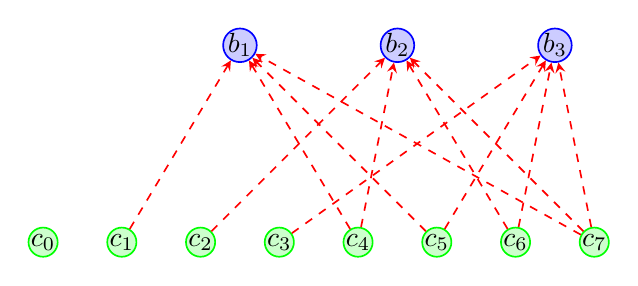
\begin{tikzpicture}[->, >=stealth, auto, semithick, edge_style/.style={color=red, dashed}]
			% Set the positions of the nodes
			\node[circle, draw=blue, fill=blue!20, inner sep=0pt] (b1) at (1.5,2.5) {$b_1$};
			\node[circle, draw=blue, fill=blue!20, inner sep=0pt] (b2) at (3.5,2.5) {$b_2$};
			\node[circle, draw=blue, fill=blue!20, inner sep=0pt] (b3) at (5.5,2.5) {$b_3$};
			
			\node[circle, draw=green, fill=green!20, inner sep=0pt] (c0) at (-1,0) {$c_0$};
			\node[circle, draw=green, fill=green!20, inner sep=0pt] (c1) at (0,0) {$c_1$};
			\node[circle, draw=green, fill=green!20, inner sep=0pt] (c2) at (1,0) {$c_2$};
			\node[circle, draw=green, fill=green!20, inner sep=0pt] (c3) at (2,0) {$c_3$};
			\node[circle, draw=green, fill=green!20, inner sep=0pt] (c4) at (3,0) {$c_4$};
			\node[circle, draw=green, fill=green!20, inner sep=0pt] (c5) at (4,0) {$c_5$};
			\node[circle, draw=green, fill=green!20, inner sep=0pt] (c6) at (5,0) {$c_6$};
			\node[circle, draw=green, fill=green!20, inner sep=0pt] (c7) at (6,0) {$c_7$};
			% Draw the edges
			
			\draw[edge_style] (c1) -- (b1);
			\draw[edge_style] (c2) -- (b2);
			\draw[edge_style] (c3) -- (b3);
			\draw[edge_style] (c4) -- (b1);
			\draw[edge_style] (c4) -- (b2);
			\draw[edge_style] (c5) -- (b1);
			\draw[edge_style] (c5) -- (b3);
			\draw[edge_style] (c6) -- (b2);
			\draw[edge_style] (c6) -- (b3);
			\draw[edge_style] (c7) -- (b1);
			\draw[edge_style] (c7) -- (b2);
			\draw[edge_style] (c7) -- (b3);
			% Position the parts
		\end{tikzpicture}
	\end{center}
	\caption{
		\picod
		کامل برای
		$m = 3$
	}
	\label{figure:complete_instance}
	
\end{figure}
\begin{theorem}
	\label{thm:hardexam1}
	نمونه‌ای از 
	\picod
	وجود دارد که به حداقل
	$\Omega(\log(n))$
	ارسال نیاز دارد.
\end{theorem}
\begin{proof}
	برای هر
	$n$
	یک 
	\picod
	کامل با
	$n$
	گیرنده می‌سازیم. در یک 
	\picod
	کامل فرستنده می‌تواند با ارسال
	$m = \log(n)$
	پیام همه‌ی گیرنده‌ها را ارضا کند(تمام پیام‌ها را ارسال کند.). حال کافی است نشان دهیم که بهتر از این کران وجود ندارد.
	
	با استقرا روی رتبه ماتریس کدگذاری 
	$A$
	نشان می‌دهیم که رتبه ماتریس باید حداقل 
	$m$
	باشد تا طبق
	\autoref{lemma:algebraicconstraint}
	گیرنده‌ها بتوانند ارضا شوند.
	
	فرض کنید
	$J \subseteq [m]$
	مجموعه‌ی اندیس تعدادی از ستون ها باشد. به ازای هر
	$J$
	یک گیرنده هست که 
	$R_j = J$
	یعنی اندیس ستون‌های زیر ماتریس
	$A_{R_j}$
	که گیرنده‌ی
	$c_j$
	از آن برای بازیابی یک متغیر استفاده می‌کند برابر
	$J$
	باشد. در یک نمونه از
	\picod
	کامل، برای هر
	$J$
	ای 
	\autoref{lemma:algebraicconstraint}
	باید برقرار باشد زیرا به ازای هر
	$b_i$
	یک گیرنده هست که دقیقا همان متغیر را باید بازیابی کند(
	گیرنده با اطلاعات جانبی
	$S_j = [m] \setminus \{i\}$
	). برای
	$J = \{j_1\}$
	برای این‌که گیرنده‌ای که دقیقا باید همان متغیر را بازیابی کند ارضا شود ستون
	$j_1$
	نباید صفر باشد. پس: 
	$\forall J, |J| = 1 \Rightarrow rank(A_J) = 1$
	. برای
	$|J| = 2$
	هر دو ستون متفاوت ماتریس باید مستقل خطی باشند. در غیر این صورت اگر
	$J = \{j_1, j_2\}$
	مستقل خطی نباشند، در این صورت گیرنده‌
	$c_k$
	که
	$R_k = \{j_1, j_2\}$
	نمی‌تواند هیچ کدام از 
	$b_{j_1}, b_{j_2}$
	را بازیابی کند. پس 
	$\forall J, |J| = 2 \Rightarrow rank(A_J) = 2$
	. حال برای فرض استفرا، فرض کنید
	$\forall J, |J| = l \Rightarrow rank(A_J) = l$
	حال برای
	$|J| = l + 1$
	اگر تمام گیرنده‌هایی که
	$l + 1$
	پیام را ندارند یعنی
	$|R_k| = m - l - 1 $
	ارضا می‌شوند پس برای یک
	$i \in J$
	داریم
	$\alpha_i \notin span(A_{J \setminus \{i\}})$
	پس
	$\rank(A_{J}) = \rank(\alpha_i) + \rank(A_{J \setminus \{i\}}) = 1 + l$
\end{proof}
\section{الگوریتم‌های تصادفی}
\subsection{\lr{GRCOV} }
\picod
ذات بسیار متفاوتی نسبت به
\icod
دارد. مثلا زمانی که یکی از متغیرها در مجموعه‌ی اطلاعات جانبی هیچ کدام از گیرنده‌ها نباشد تنها با یک ارسال می‌توان تمام گیرنده‌ها را ارضا کرد در حالی که در
\icod
این کد با طول یک، کد درستی نیست. در واقع بر خلاف
\icod
که هر تک گیرنده ممکن است به خاطر پیامی که می‌خواهد بازیابی کند طول کد را افزایش دهد در
\picod
گیرنده‌ها برهمکنش بیشتری روی طول کد دارند. به عنوان مثالی دیگر زمانی که اطلاعات جانبی تعدادی از گیرنده‌ها شامل تمام متغیرها به جز یکی است فرشتنده کافی است مجموع تمام متغیرها را ارسال کند. 

ایده‌ی اصلی الگوریتم‌های
\lr{GRCOV1 \& GRCOV2}
 پیدا کردن مجموعه‌هایی از گیرنده‌ها است که ویژگی‌های بالا را داشته باشند.
 
 \begin{remark}
 	در مقاله
 	\cite{pliablefirstpaper}
 	نمادگذاری گراف اطلاعات جانبی بر خلاف نمادگذاری مرسوم این حوزه و این پایان‌نامه است. در واقع در مقالات بعدی این نمادگذاری تغییر کرد. در این مقاله اگر
 	$j \notin S_i$
 	آنگاه بین
 	$b_j$
 	و
 	$c_i$
 	یالی قرار دارد که برعکس نمادگذاری مرسوم است.
 \end{remark}
 
 فرض کنید برای دو متغیر
 $b_{\sigma_1}$
 و
 $b_{\sigma_2}$
 \footnote{
 همان طور که در
 \autoref{remark:xbdiff}
 گفته شد 
 $b_{\sigma_1}$
 واقعا متغیر تصادفی نیست بلکه راس متناظر متغیر
 $X_{\sigma_1}$
 است.
 }
 همسایه‌های این دو راس
 $N[b_{\sigma_1}] \cup N[b_{\sigma_2}]$
 را بر اساس تعداد همسابه‌های خود در بخش
 $B$
 گراف به دو دسته تقسیم می‌کنیم. دسته اول راس‌های
 $c_i$ای
 که به همه به جز یکی وصل‌اند. در واقع به
 $W_1(B_1)$
 که در
 \autoref{def:nonnei}
 تعریف کردیم توجه می‌کنیم. حال اگر
  $Y_1 = \bigoplus\limits_{b \in B_1} b$
  را فرستنده ارسال کند تمام اعضای
  $W_1(B_1)$
  می‌توانند با اطلاعات جانبی خود پیام جدیدی را با کم کردن اطلاعات جانبی خود از
  $Y_1$
  بازیابی کنند.
  
 با توجه به بحث قبلی در الگوریتم
\GRCOVone
به دنبال مجموعه‌ای از رئوس گراف مانند
$B_1$
هستیم که 
$|W_1(B_1)|$
بیشینه باشد. به جای این‌که در هر گام مجموعه‌ای با اندازه‌ی ماکسیمم پیدا کنیم به صورت حریصانه مجموعه‌ای با اندازه‌ی ماکسیمال پیدا می‌کنیم.

به مجموعه‌ی 
$B_1 = \{b_{v_1}, \ldots, b_{v_t}\}$
می‌گوییم ماکسیمال اگر برای هر راس
$b_{v_{t  +1}} \notin B_1$
داشته باشیم:
\begin{equation}
	\tag{شرط ماکسیمال بودن}
	|W_1(B_1 \cup \{b_{v_{t + 1}} \})| < |W_1(B_1)|
\end{equation}

برای پیدا کردن یک مجموعه‌ی ماکسیمال با یک مجموعه‌ی تهی شروع می‌کنیم و در هر گام یک راس جدید را به صورت حریصانه به طوری که 
$|W_1(B_1)|$
را بیشینه کند انتخاب می‌کنیم. این کار را تا زمانی که نتوانیم ادامه بدهیم انجام می‌دهیم.

زمانی که مجموعه‌ی ماکسیمال را پیدا کردیم مطابق آنچه قبل‌تر گفته شد پیام
 $Y_1 = \bigoplus\limits_{b \in B_1} b$
 را به کد خود اضافه می‌کنیم(فرستنده این پیام را هم ارسال می‌کند). سپس تمام راس‌های
 $B_1$
 و
 $w_1(B_1)$
 از گراف حذف می‌شوند و دوباره همین کار را تکرار می‌کنیم. در نهایت پس از 
 $s$
 گام کد نهایی برابر
 $Y = (Y_1, \ldots, Y_s), Y_i =  \bigoplus\limits_{b \in B_i} b$
 خواهد بود. این الگوریتم
 \GRCOVone\footnote{\lr{greedy cover}}
 	نام دارد. زمان اجرای این الگوریتم برابر
 	$O(mn^2)$
 	است.
 	\begin{algorithm}
 		\caption{
 			پوشش حریصانه‌ی
 			\lr{GrCov($G,m,n,t$) }
 			\cite{pliable2015paper}}
 		\label{algorithm:grcov}
 		\begin{algorithmic}[1]
 			\Require
 			گراف اطلاعات جانبی
 			$G$
 			با
 			$n$
 			گیرنده و
 			$m$
 			پیام برای مسئله‌ی
 			\picodtt{t}
 			
 			\Ensure
 			یک کد اندیس منعطف برای
 			$G$
 			\State 
 			قرار دهید
 			$\mathcal{C} = \{\}$
 			\State برای هر
 			 $\forall i \in [n]$
 			 قرار دهید
 			 $CNT[i] = t$ 
 			\While{
 				$i$
 				وجود دارد که
 				 $CNT[i] \neq 0$
 				 }
		 			\State
		 			قرار دهید
		 			 $B \leftarrow \varnothing$.
		 			\While{$B$
		 			یک مجموعه‌ی ماکسیمال نیست}
				 			\State
				 			راس
				 			 $b_v \notin B$ 
				 			 که
				 			 $\left|W_1\left(B \cup\left\{b_v\right\}\right)\right|$
				 			 بیشینه باشد را بیابید.
				 			\State قرار دهید
				 			$B \leftarrow B \cup\left\{b_v\right\}$
		 			\EndWhile
		 			\State قرار دهید
		 			 $\mathcal{C} \leftarrow \mathcal{C} \cup\left\{\sum_{u=1}^{|B|} b_{v_u}, b_{v_u} \in B\right\}$
		 			\For{ $c_i \in W_1(B)$ }
		 			\If{
		 				$c_i$ 
		 				به
		 		$b_j \in B$
		 		متصل است
		 	}
		 	\State یال متناظر در
		 	 $G$
		 	 را حذف کنید.
		 	 \EndIf
		 			\State قرار دهید $CNT[i] \leftarrow CNT[i]-1$.
		 			\EndFor
 			\EndWhile
 			\State کد
 			 $\mathcal{C}$
 			 را به عنوان خروجی برگردانید.
 		\end{algorithmic}
 	\end{algorithm}

 الگوریتم
 	\lr{GRCOV2} 
 	تغییر کوچکی نسبت به الگوریتم قبلی دارد. در الگوریتم قبلی وقتی یک مجموعه‌ی ماکسیمال را پیدا می‌کردیم هم
 $B_1$
 و هم متغیرهای مربوطه یعنی
 $w_1(B_1)$
 را حذف می‌کردیم. ولی ممکن است که این متغیرها در پیدا کردن مجموعه‌های ماکسیمال بهتری به ما کمک کنند. در این الگوریتم تنها
 $B_1$
 را حذف می‌کنیم.
 
 زمان اجرای این الگوریتم نیز
 $O(mn^2)$
 است.
 \subsection{\lr{SETCOV}}
 فرگولی و براهما برای آزمایش کارایی الگوریتم‌های بالا، الگوریتم
 \lr{SETCOV}
 را معرفی می‌کند. این الگوریتم بر مبنای کاهش مسئله به
 \icod
 طراحی شده است. در 
 \picod
 هر گیرنده 
 $i$
 با بازیابی هر پیام از
 $R_i$
 ارضا می‌شود. برای تبدیل یک نمونه از
 \picod
 به
 \icod
 به ازای هر گیرنده
 $R_i$
 شبه‌گیرنده 
 $c_{i, 1}, \ldots, c_{i, {R_i}}$
 قرار می‌دهیم که هر کدام به دنبال یکی پیام‌های
 $R_i$
 است و اطلاعات جانبی مشابهی مانند
 $c_i$
 دارد. در نتیجه 
 \icod
 نهایی 
 $\sum\limits_{i = 1}^{n} |R_i|$
 گیرنده خواهد داشت. این نمونه توسط هر کدام از الگوریتم‌های
 \icod
 قابل حل است. فرگولی از بین الگوریتم‌های ارائه شده در
 \cite{25}
 ساده‌ترین آن‌ها که بر مبنای
 \transf{پوشش خوشه‌ای حریصانه}{greedy clique cover}
 است را استفاده می‌کند.
 
 پس از حل مسئله‌ی
 \icod
 ایجاد شده فرض کنید 
 $Y$
 کد خروجی الگوریتم پوشش خوشه‌ای حریصانه باشد. در این الگوریتم هر گیرنده تنها با استفاده از یک از پیام‌ها، پیام مورد نظر خود را بازیابی می‌کند. در واقع هر پیام توانایی بازیابی تنها با استفاده از همان پیام را به تعداد از گیرنده‌ها می‌دهد. این مسئله باعث می‌شود به طورر طبیعی یک رابطه‌ی "پوشش" دادن بین اعضای کد و گیرنده‌ها(در اینجا شبه‌گیرنده‌ها) ایجاد شود به این صورت که هر عضو کد تعداد از گیرنده‌ها را پوشش می‌دهد. چون هدف اصلی ما گیرنده‌های
 \picod
 هستند و نه شبه‌گیرنده‌هایی که ساخته‌ایم این برای هر عضو کد پوشش را به صورت گیرنده‌هایی که ارضا می‌کند تعریف می‌کنیم. یعنی اگر
 $Y_t$
 شبه‌گیرنده‌های
 $c_{\sigma_1, g_1}, \ldots, c_{\sigma_s, g_s}$
 را ارضا می‌کند تعریف می‌کنیم:
 $$C(Y_t) =\{ c_{\sigma_1}, c_{\sigma_1}\}$$
 طبیعی است که هر گیرنده ممکن است در چندین مجموعه‌ی مختلف باشد. برای پیدا کردن یک جواب برای
 \picod
 تنها کافی است تعداد از 
 $C(Y_i)$
 ها را پیدا کنیم که کل گیرنده‌ها را پوشش دهند و در بین جواب‌ها دنبال جواب با کم‌ترین تعداد مجموعه‌‌ایم. این یک نمونه از مسئله‌ی معروف
 \transf{پوشش مجموعه‌ای}{SET-COVER}
 است که عناصر، گیرنده‌ها هستند و مجموعه‌ها پوشش‌های
 $C(Y_i)$.
 
 فرگولی در پیاده سازی آزمایشگاهی از روش استاندارد حریصانه تقریبی برای این مسئله استفاده می‌کند که زمان اجرای نهایی آن
 $O(m^2 n^6)$
 است.
\subsubsection{k-GRCOV}
برای حالت
\picodt
یک تعمیم طبیعی از الگوریتم قبلی وجود دارد. به جای این‌که در هر گاه راس‌هایی که یک پیام جدید را بازیابی می‌کنند حذف کنیم، هر راس 
$c_i$
یک شمارنده برابر
$\min(k, |R_i|)$
دارد و در هر گام که یک راس یک پیام جدید را بازیابی می‌کند این شمارنده را یک واحد کم می‌کنیم و راس‌های
$w_1(B_j)$
را به راس
$c_i$
به عنوان اطلاعات جانبی وصل می‌کنیم. هر راسی که شمارنده‌اش به صفر برسد را هم حذف می‌کنیم. زمان اجرای این الگوریتم
$O(kmn^2)$
است.

\subsection{
نتایج عددی
}
فرگولی و براهما  الگوریتم‌های گفته شده را به صورت عملی روی نمونه‌های تصادفی از مسئله تست می‌کنند. در این آزمایش‌ها 
$n = m = 500$
و هر یال در گراف اطلاعات جانبی را هم با احتمال
$p$
قرار می‌دهند. یعنی هر گیرنده با احتمال
$p$
ان پیام‌ را از قبل می‌داند. همچنین برای مقایسه بهتر، در نمونه‌های تولیدی هر گیرنده می‌خواهد یک پیام متفاوت را در مسئله‌ی
\icod
بازیابی کند.
\begin{figure}
	\centering
	\includegraphics[width=0.7\linewidth]{figs/ch3/pliable2012}
	\caption{\cite{pliablefirstpaper}}
	\label{fig:pliable2012}
\end{figure}

در 
\autoref{fig:pliable2012}
کاراریی الگوریتم‌های مختلف به ازای 
$p$
های مختلف آمده است. برای هر
$p$
بیش از هزار بار آزمایش تکرار شده است. همان طور که در شکل مشخص است تفاوتی چشمگیر بین الگوریتم‌های
\picod
و الگوریتم‌های مختلف
\icod
است(تفاوتی چشمگیری بین الگوریتم‌های مختلف
\icod
که در این مقایسه مهم باشد دیده نمی‌شود). در حالی که الگوریتم‌های گفته شده‌ی
\picod
به طور میانگین کمتر از
$11$
پیام ارسال می‌کنند الگوریتم‌های
\icod
تنها وقتی
$p \geq 0.95$
است این کاراریی را دارد. یعنی زمانی که گراف اطلاعات جانبی بسیار پر است.

در بین الگوریتم‌های بیان شده
\lr{GRCOV2}
بهترین عملکرد را دارد و
\lr{GRCOV1}
با فاصله‌ی کمی از آن عمل می‌کند.

الگوریتم
\lr{SETCOC}
روند جالبی دارد. در محدوده‌ی 
$p \leq 0.5$
بهتر از
\lr{GRCOV2}
عمل می‌کند. بخشی از این عملکرد را می‌توان این گونه توجیه کرد که برای مقادیر کم
$p$
گراف اطلاعات جانبی تنک می‌شود و در نتیجه هر عضو کد(پیام ارسال شده توسط فرستنده)  برای تعداد بیشتری گیرنده حاوی اطلاعات(آنتروپی شرطی(بر پایه اطلاعات جانبی هر گیرنده)) است و در نتیجه وقتی به دنبال پوشش هستیم هر مجموعه گیرنده‌های بیشتری را شامل می‌شود.

همان طور که در
\autoref{fig:pliable2012}
می‌بینید بیشینه‌ی طول کد در الگوریتم
\lr{GRCOV2}
در آزمایش‌های انجام شده برای تمام نمونه‌های
\picod
کمتر از
$\log(500) \approx 6$
است. در شکل
\autoref{fig:pliable20122}
به ازای مقادیر محتلف 
$n$
(که همچنان
$m = n$
) و نمونه‌های تصادفی یونیفرم می‌بینیم که برای
$n \geq 60$
طول کد حداکثر
$\log(n)$
است.

نتایج اجرای الگوریتم
\lr{k-GRCOV2}
در 
\autoref{fig:pliable20123}
آمده است. همان طور که مشخص است در عمل به طور میانگین با کدهای با طول کمتر از
$17$
می‌توان 
$500$
گیرنده که به دنبال بازیابی 
$5$
هستند را ارضا کرد.
\begin{figure}
	\centering
	\includegraphics[width=0.7\linewidth]{figs/ch3/pliable2012_2}
	\caption{\cite{pliablefirstpaper}}
	\label{fig:pliable20122}
\end{figure}
\begin{figure}
	\centering
	\includegraphics[width=0.7\linewidth]{figs/ch3/pliable2012_3}
	\caption{\cite{pliablefirstpaper}}
	\label{fig:pliable20123}
\end{figure}

\subsection{\lr{RANDCOV}}
\subsubsection{\lr{RANDCOV}}
این الگوریتم روند اثبات
\autoref{theorem:log1}
را برای پیدا کردم کدگذاری دنبال می‌کند. گیرنده‌ها به حداکثر
$g = O(\log(m))$
گروه ناتهی
$S_1, \ldots, S_g$
افراز می‌شوند به طوری که نسبت حداکثر و حداقل درجه در هر گروه حداکثر یک ثابت مشخص
$r$
باشد. فرض کنید بزرگترین درجه موثر در
$S_i$
برابر
$d_{max, i}$
باشد. در همسایگی
$N[S_i]$
هر راس را با احتمال
$p_i = \dfrac{1}{d_{max, i}}$
 انتخاب می‌کنیم.
 اگر
 $B_i$
 مجموعه‌ی راس‌های انتخابی باشد،
 گیرنده‌های مجموعه‌ی
 $W_1(B_i)$
 ارضا می‌شوند. این گیرنده‌ها را حذف می‌کنیم و فرآیند را تا زمانی که تمام گیرنده‌های
 $S_i$
 ارضا شوند ادامه می‌دهیم. تعداد مجموعه‌های تصادفی انتخاب شده مورد نیاز برابر طول کد خواهد بود. این کار را برای تمام مجموعه‌های
 $S_1, \ldots, S_g$
 انجام می‌دهیم. پیاده سازی ساده‌ای از این الگوریتم زمان اجرای
 $O(m n \log(n))$
 
 \subsubsection{\lr{RANDCOV-PP}}
 گرچه طول کد ساخته شده در الگوریتم
 \lr{RANDCOV}
 توسط
 \autoref{theorem:log1}
 محدود می‌شود، همان طور که در 
 \autoref{subsection:numerical}
  خواهیم دید، یک پیاده سازی ساده بدون هیچ تغییری خروجی خوبی نسبت به
  \lr{GRCOV}
  نخواهد داشت. برای بهبود این الگوریتم می‌توانیم از مرحله‌ی پس‌پردازش زیر استفاده می‌کنیم. فرض کنید
  $B_1$
  و
  $B_2$
  دو مجموعه از گیرنده‌ها باشند. اگر هیچ یالی از
  $B_1$
  به
  $W_1(B_2)$
  نداشته باشد و همچنین هیچ یالی از
  $B_2$
  به
  $W_1(B_1)$
  وجود نداشته باشد آنگاه می‌توانیم با ارسال جمع تمام پیام‌های
  $B_1 \cup B_2$
  تمام گیرنده‌های
  $W_1(B_1) \cup W_1(B_2)$
  را ارضا کنیم. این ایده تنها به دو مجموعه وابسته نیست و می‌توان به هر تعداد مجموعه با شرایط گفته شده تعمیم داد. در هر مرحله به صورت حریصانه بیشترین تعداد مجموعه که در شرط بالا صدق می‌کنند را انتخاب می‌کنیم. این الگوریتم همچنان در زمان
  $O(m n \log(n))$
  اجرا می‌شود.
  \subsection{
  نتایج عددی
  }
  \label{subsection:numerical}
  در
  \autoref{fig:pliable2015}
  نتایج شبیه‌‌سازی‌های الگوریتم‌های گفته شده را مشاهده می‌کنید. در این شبیه سازی‌ها عداد گیرنده‌ها و پیام‌ها برابر
  $n = m = 512$
  است و میدان
  $\mathbb{F}_2$
  استفاده شده است. برای الگوریتم‌های
  \lr{RANDCOV}
  و
  \lr{RANDCOV-PP}
  نیز
  $r = 3$
  انتخاب شده است. برای ساخت هر نمونه از مسئله از روش زیر استفاده کردیم. هر گیرنده با احتمال
  $p_{msg}$
  هر کدام از پیام‌ها را ممکن است در اطلاعات جانبی خود داشته باشد. این مدل از ساخت نمونه می‌تواند مدلی برای 
  \lr{block-fading}
  در 
  \transf{
  کانال‌های بی‌سیم
}{wireless channels}
   باشد یعنی زمانی که نسبت 
   \transf{
   پیام به نویز
}{channel SNR =  channel signal to noise ratio}
کم باشد، مثلا لایه‌های بالایی شبکه با احتمال
$1 - p_{msg}$
پیام‌ها را پاک کنند.
\autoref{fig:pliable2015a}
میانگین کارایی الگوریتم‌ها بر روی نمونه‌های مختلف را نشان می‌دهد. برای هر 
$p_{msg}$
بیش از ده هزار نمونه با ساخته شده است و طول کد میانگین روی تمام نمونه‌ها محاسبه شده است.

همان طور که انتظار می‌رفت تفاوت بسیار زیادی بین کارایی(طول کد) در الگوریتم‌ها
\picod
و
\icod
وجود دارد. در حالی که هر الگوریتم‌های
\picodtt{1}
کدی با طول کمتر از ۲۶ تولید می‌کنند، طول کد برای
\icod
تنها زمانی در این بازی قرار می‌گیرد که
$p_{msg} \geq 0.87$
باشد، یعنی زمانی که گراف اطلاعات جانبی افراد بسیار
\transf{
	متراکم
}{
dense
}
  باشد.
  
  در بین الگوریتم‌های 
  \picod
  \lr{GRCOV}
  بهترین کارایی را دارد. در واقع
    \lr{GRCOV}
     به صورت نظری روی نمونه‌های تصادفی، کارایی مشابهی به صورت 
     \transf{
     تقریبی
    }{asymptotic}
    با
    \lr{RANDCOV}
    دارد ولی در عمل کارایی بسیار بهتری دارد.
    
    برای بررسی کارایی
        \lr{GRCOV}
        در حالت چند پیامه
        \picodtt{t}
        نمونه‌های تصادفی با
        $p_{msg} = 0.5$
        و مقادیر متفاوت
        $t$
        و
        $n$
        و
        $m = n$
        ساخته شده است. اگر در یک نمونه‌ تصادفی
        $m - |S_i| < t$
        در این صورت مطابق تعریف این گیرنده به دنبال بازیابی
        $m - |S_i|$
        پیام است. در
        \autoref{fig:pliable2015b}
        به ازای مقادیر مختلف
        $t$
        و چند مقدار مختلف
        $n$
        کارایی الگوریتم به تصویر کشیده شده است.
        
        برای هر
        $n$
        بعد از کمی فاز ابتدایی، طول کد به صورت خطی نسبت به
        $t$
        افزایش می‌یابد. این نتیجه را به خاطر
        \autoref{thm:pliable2015_8}
        انتظار داشتیم. همچنین خط‌های نمودار در
                \autoref{fig:pliable2015b}
                برای
                $t > 5$
                به صورت تقریبا موازی هستند یعنی طول کد نسبت به 
                $n$
                مستقل است. که با نتیجه‌ی
                $O(t + \log^2(n))$
                برای
                $t$
                های بزرگ مطابقت دارد. خط‌های نشان دهنده‌ی خطا(حداکثر و حداقل طول کد در نمونه‌ها) نیز مشابها روندی خطی را دنبال می‌کنند.
                
                در
                \autoref{fig:pliable2015c}
                مطابق
                  \autoref{fig:pliable2015b}
                  است ولی این بار
                  $n$
                  در محور افقی آمده است و به ازای مقدارهای مختلف
                  $t$
                  نمودار رسم شده است.
                  
                  در
                    \autoref{fig:pliable2015d}
                    تاثیر
                    $p_{msg}$
                    را بررسی می‌کنیم. این نمودار به ازای
                    $m = n = 100$
                    و مقادیر مختلف
                    $t$
                    رسم شده است.
  \begin{figure}
  	\centering
	\begin{subfigure}[b]{0.45\textwidth}
			\centering
  	\includegraphics[width=\textwidth]{figs/ch3/pliable2015_a}
			\caption{}
			\label{fig:pliable2015a}
		\end{subfigure}
		\hfill
		  \begin{subfigure}[b]{0.45\textwidth}
			\centering
			\includegraphics[width=\textwidth]{figs/ch3/pliable2015_b}
			\caption{}
			\label{fig:pliable2015b}
		\end{subfigure}
		\\
		\begin{subfigure}[b]{0.45\textwidth}
			\centering
			\includegraphics[width=\textwidth]{figs/ch3/pliable2015_c}
			\caption{}
			\label{fig:pliable2015c}
		\end{subfigure}
		\hfill
		\begin{subfigure}[b]{0.45\textwidth}
			\centering
			\includegraphics[width=\textwidth]{figs/ch3/pliable2015_d}
			\caption{}
			\label{fig:pliable2015d}
		\end{subfigure}
		  	\caption][
		  	مقایسه‌ی الگوریتم‌های تصادفی
		  	]{
		  		مقایسه‌ی الگوریتم‌های تصادفی
		  		\cite{pliable2015paper}
		  		}
		\label{fig:pliable2015}
  \end{figure}

\section{
	الگوریتم قطعی
	\lr{BinGreedy}
	}
	\subsection{
	توصیف الگوریتم
	}

در الگوریتم قطعی‌ای که معرفی خواهیم کرد از دو مفهوم گیرنده‌های موثر و درجه موثر استفاده می‌کنیم. برای یک پیام
$X_i$
(یا معادلا راس
$b_j$
)
به گیرنده‌هایی که می‌خواهیم این پیام را بازیابی کنند، گیرنده‌های موثر می‌گوییم. همچنین درجه موثر یک پیام تعداد گیرنده‌هایی است که آن پیام دارد. با استفاده از این مفاهیم پیام‌های را به گروه‌هایی تقسیم می‌کنیم که درجه موثر مشابهی دارند. سپس نشان می‌دهیم که به دلیل منظم بودن درجه با ارسال‌هایی که صرفا بر اساس پیام‌های هر گروه است می‌توانیم ضریب ثابتی از گیرنده‌های موثر هر گروه را ارضا کنیم.

در هر گام الگوریتم
\lr{binary field greedy (BinGreedy)}
دو مرحله وجود دارد. مرحله مرتب سازی و مرحله‌ی ارسال حریصانه. در مرحله مرتب سازی بر اساس مفهوم پیام‌ها را به صورت کاهشی بر اساس درجه‌ی موثر آن‌ها مرتب می‌کنیم سپس پیام‌ها را به 
$\log(n)$
گروه افراز می‌کنیم. در مرحله‌ی ارسال ترکیب خطی‌ای از پیام‌های هر گروه را در نظر گرفته و برای هر گروه دو ارسال انجام می‌دهیم. در نتیجه
$2 \log(n)$
ارسال در کل خواهیم داشت.

\begin{definition}
	[گیرنده‌ی موثر و درجه موثر]
	برای یک جایگشت داده‌شده‌ی 
	$\pi = (j_1, \ldots, j_m)$
	از پیام‌ها، درجه موثر
	$b_{j_l}$
	ناظر به جایگشت 
	$\pi$
	را برابر تعداد همسایه‌های 
	$b_{j_l}$
	(چون گراف دو بخشی است برابر گیرنده‌هایی که در گراف به آن یال دارند خواهد بود)	که به هیچ یک از راس‌‌های پیام ما قبل آن یعنی
	$b_{j_1}, \ldots, b_{j_{l - 1}}$
	متصل نیستند تعریف می‌کنیم. همچنین به راس‌هایی که در درجه‌ی موثر راس
		$b_{j_l}$
		شمرده شده‌اند راس‌های موثر این راس ناظر به جایگشت
		$\pi$
		راس‌های موثر این راس ناظر به
		$\pi$
		 می‌گوییم.
		 
		 همسایه‌های
		 $b_j$
		 را با
		 $N[j]$
		 نشان می‌دهیم همچنین تعریف می‌کنیم
		 $N[j_1, \ldots, j_{l - 1}] = N[j_1] \cup \ldots \cup N[j_{l - 1}]$
		 . راس‌های موثر
 		$b_{j_l}$
 		را با
 		$N^\dagger_\pi [j_l] = N[j_l] \setminus N[j_1, \ldots, j_{l - 1}]$
 		نشان می‌دهیم همچنین درجه را با
 		$d^\dagger_\pi[j_l] = |N^\dagger_\pi [j_l] |$
 		نشان می‌دهیم.
\end{definition}

توجه کنید که درجه موثر و راس‌های موثر یک راس وابسته به جایشگت هستند.

\begin{example}
	در شکل
	\autoref{figure:example:effective}
	با جایگشت
	$<b_1, b_2, b_3>$
	داریم:
	\begin{align*}
			&d^\dagger[1] = 4, N^\dagger[1] = \{1, 4, 5, 7\} \\
			&d^\dagger[2] = 2, N^\dagger[1] = \{2, 6\} \\
			&d^\dagger[3] = 1, N^\dagger[1] = \{3\}
	\end{align*}

	\begin{figure}
		\begin{center}
			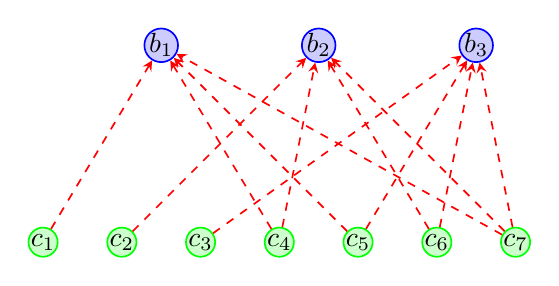
\begin{tikzpicture}[->, >=stealth, auto, semithick, edge_style/.style={color=red, dashed}]
				% Set the positions of the nodes
				\node[circle, draw=blue, fill=blue!20, inner sep=0pt] (b1) at (1.5,2.5) {$b_1$};
				\node[circle, draw=blue, fill=blue!20, inner sep=0pt] (b2) at (3.5,2.5) {$b_2$};
				\node[circle, draw=blue, fill=blue!20, inner sep=0pt] (b3) at (5.5,2.5) {$b_3$};
				
				\node[circle, draw=green, fill=green!20, inner sep=0pt] (c1) at (0,0) {$c_1$};
				\node[circle, draw=green, fill=green!20, inner sep=0pt] (c2) at (1,0) {$c_2$};
				\node[circle, draw=green, fill=green!20, inner sep=0pt] (c3) at (2,0) {$c_3$};
				\node[circle, draw=green, fill=green!20, inner sep=0pt] (c4) at (3,0) {$c_4$};
				\node[circle, draw=green, fill=green!20, inner sep=0pt] (c5) at (4,0) {$c_5$};
				\node[circle, draw=green, fill=green!20, inner sep=0pt] (c6) at (5,0) {$c_6$};
				\node[circle, draw=green, fill=green!20, inner sep=0pt] (c7) at (6,0) {$c_7$};
				% Draw the edges
				
				\draw[edge_style] (c1) -- (b1);
				\draw[edge_style] (c2) -- (b2);
				\draw[edge_style] (c3) -- (b3);
				\draw[edge_style] (c4) -- (b1);
				\draw[edge_style] (c4) -- (b2);
				\draw[edge_style] (c5) -- (b1);
				\draw[edge_style] (c5) -- (b3);
				\draw[edge_style] (c6) -- (b2);
				\draw[edge_style] (c6) -- (b3);
				\draw[edge_style] (c7) -- (b1);
				\draw[edge_style] (c7) -- (b2);
				\draw[edge_style] (c7) -- (b3);
				% Position the parts
			\end{tikzpicture}
		\end{center}
		\caption{
			\picod
			مثالی برای درجه موثر و راس‌های موثر
		}
		\label{figure:example:effective}
		
	\end{figure}
\end{example}

حال به توصیف گام‌های الگوریتم می‌پردازیم.
\begin{itemize}
	\item[مرحله‌ی مرتب سازی] 
	
	در این مرحله
		\begin{enumerate}
			\item [گام اول]
			در گراف اصلی که با
			$G_1$
			نشان می‌دهیم راس پیام
			$j_1$
			با درجه بیشینه را در نظر بگیرید. در صورت وجود چند گزینه یکی را به دلخواه انتخاب کنید. خواهیم داشت
			$\forall j \in [m] \setminus \{j_1\} |N[j_1]| \geq |N[j]|$
			\item [گام دوم]
			زیر گراف القا شده توسط راس‌های پیام
			$[m] \setminus \{j_1\}$
			و راس‌های گیرنده‌ی
			$[n] \setminus N[j_1]$
			را با
		   $G_2$
		   نمایش می‌دهیم. حال مشابه گام قبل راس پیام
		   $j_2$
		   با درجه بیشینه را در نظر می‌گیریم. خواهیم داشت:
		   $\forall j \in [m] \setminus \{j_1, j_2\} |N_{G_2}[j_2]| \geq |N_{G_2}[j]|$
		   که
		   $N_{G_2}[j] = N[j] \cap V(G_2) = N[j] \setminus N[j_1]$
			\item [
			گام 
			$l$
			ام
			]
			در گام
			$l = 3, \ldots, m$
			گراف القا شده توسط راس‌های پیام
			$[m] \setminus \{j_1, \ldots, j_{l - 1}\}$
			و راس‌های گیرنده‌ی
			$[n] \setminus N[j_1, \ldots, j_{l-1} ]$
			را با
			$G_l$
			نمایش می‌دهیم. راس پیام
			$j_l$
			را مشابه قدم‌های قبل با بیشنه درجه در زیر گراف
			$G_l$
			 انتخاب می‌کنیم. خواهیم داشت:
			 $\forall j \in [m] \setminus \{j_1, \ldots, j_l\}: |N_{G_l}[j_l]| \geq |N_{G_l} [j]|$
			 که
			 $N_{G_l} = N[j] \cap V(G_l) = N[j] \setminus N[J_1, \ldots, j_{l - 1}] $
			
			اگر جایگشت انتخابی راس‌های ما طبق فرایند بالا باشد درجه موثر 
			$j_1$
			برابر
			$|N[j_1]|$
			 خواهید بود. به طور کلی درجه اثر گذاری راس
			 $j_l$
			 برابر
			 $|N[j_l]]\setminus N[j_1, \ldots, j_{l-1}]|$
			 خواهد بود.
			 
			 پس از انتخاب جایگشت به روش بالا، راس‌ها را بر اساس درجه موثر آن‌ها به
			 $\log(n)$
			 دسته 
			 $\mathcal{M}_1, \ldots, \mathcal{M}_{\log(n)}$
			 افراز می‌کنیم به گونه‌ای که برای راس
			 $j \in \mathcal{M}_s$
			 داشته باشیم:
			 $\dfrac{n}{2^{s - 1}} \geq d^\ddagger[j] > \dfrac{n}{2^s}$
			 
			 در این صورت برای پیام
			 $j$
			 در دسته‌ی
			 $\mathcal{M}_s$
			 خواهیم داشت:
			 $$d^{\ddagger}[j] > \dfrac{n}{2^s} \triangleq \dfrac{d}{2}$$
			 و همچنین:
			 $$|N[j] \cap \mathcal{N}_s| \leq \dfrac{n}{2^{s - 1}} \triangleq d$$
			 که
			 $\mathcal{N}_s$
			 مجوعه‌ی تمام گیرنده‌های موثر پیام‌های مجموعه‌ی
			 $\mathcal{M}_s$
			 است
			 $\mathcal{N}_s = \cup_{j' \in \mathcal{M}_s} N^{\ddagger}[j']$
			 نامساوی دوم به این دلیل برقرار است که اگر
			 $|N[j] \cap \mathcal{N}_s | > d$
			 در این صورت پیام
			 $j'$
			 در فرایند گروه بندی بالا، درجه‌ی موثر بزرگتر از
			 $d$
			 داشته است و در نتیجه باید در یک گروه قبل تر(با
			 $s$
			 کوچک تر) دسته بندی می‌شد.
			 
			 در مثال در
			 \autoref{figure:example:effective}
			 یک ترتیب و گروه بندی معتبر برابر است با
			 $b_1, b_2, b_3$
			 و
			 $\mathcal{M}_1 = \{1\}, \mathcal{M}_2 = \{2\}, \mathcal{M}_3 = \{3\}$
		\end{enumerate}
	\item[مرحله ارسال] 
	برای هر گروه
	$\mathcal{M}_s$
	با استفاده از یک زیر ماتریس کدگذاری با دو ردیف دو ارسال انجام می‌دهیم.
	
	در ابتدا زیر ماتریس خالی است. به ترتیب راس‌های پیام
	$\mathcal{M}_s$
	را با همان ترتیب مرحله‌ی قبل بررسی می‌کنیم و به ازای هر کدام یک ستون به زیر ماتریس اضافه می‌کنیم که به آن بردار کدگذاری می‌گوییم. بردارهای کدگذاری به یکی از سه حالت
	$\{(1, 0)^T, (0, 1)^T, (1, 1)^T\}$
	هستند. در هر گام یکی از این سه بردار را بر این اساس انتخاب می‌کنیم که بیشترین تعداد گیرنده‌های
	$\mathcal{N}_s$
	را همچنان قابل ارضا باشند. در مثال
	\autoref{figure:example:effective}
	می‌توانیم زیر ماتریس‌های کدگذاری زیر را بسازیم:
	\begin{align*}
		A_1 = \begin{bmatrix}
			1 & 0 & 0 \\
			0 & 0 & 0
		\end{bmatrix}, 
		A_2 =   \begin{bmatrix}
			0 & 1 & 0 \\
			0 & 0 & 0
		\end{bmatrix},
		A_3 =   \begin{bmatrix}
			0 & 0 & 1 \\
			0 & 0 & 0
		\end{bmatrix}
	\end{align*}
	که از کنار هم قرار دادن این زیر ماتریس‌ها به ماتریس کدگذاری زیر می‌رسیم:
		\begin{align*}
		A =  \begin{bmatrix}
			A_1\\
			A_2\\
			A_3
				\end{bmatrix}
			= \begin{bmatrix}
			1 & 0 & 0 \\
			0 & 0 & 0 \\
			0 & 1 & 0 \\
			0 & 0 & 0 \\
			0 & 0 & 1 \\
			0 & 0 & 0
		\end{bmatrix}
			\end{align*}
\end{itemize}
\subsection{شبه کد}
	\begin{algorithm}[H]
	\caption{
		الگوریتم حریصانه برای میدان دودویی
		\lr{BinGreedy($G,m,n,t$)}
		\cite{pliable2016}
		}
	\label{algorithm:bingready}
	\begin{algorithmic}[1]
		\Require
		 گراف اطلاعات جانبی
		$G$
		با 
		$n$
		گیرنده و
		$m$
		پیام برای مسئله‌ی
		\Ensure
		یک اندیس کد منعطف برای
		$G$
		\picodtt{t}
		\State 
		قرار دهید
		 $\mathcal{N} = [n]$
		\State
		قرار دهید
		 $\mathcal{C} = \{\}$
		\State
		برای هر
		 $\forall i \in [n]$
		 قرار دهید
		 $CNT[i] = t$ 
		\While{که 
			$i$
			وجود دارد که
			$CNT[i] \neq 0$
			}
		\State قرار دهید
		$B \leftarrow \varnothing$.
		\While{$B$ 
		یک مجموعه‌ی ماکسیمال نیست
		}
		\State
		راس پیام
		 $b_v \notin B$
		 را پیدا کن به طوری که
		 $\left|W_1\left(B \cup\left\{b_v\right\}\right)\right|$
		 بیشینه شود.
		\State قرار دهید
		$B \leftarrow B \cup\left\{b_v\right\}$
		\EndWhile
		\State قرار دهید
		 $\mathcal{C} \leftarrow \mathcal{C} \cup\left\{\sum_{u=1}^{|B|} b_{v_u}, b_{v_u} \in B\right\}$
		\For{ $c_i \in W_1(B)$ }
		\If{ $c_i$ 
			به
			 $b_j \in B$
			 متصل است
			 }
		\State
		یال متناظر در
		 $G$
		 را حذف کن.
		\EndIf
		\State
		قرار دهید
		 $CNT[i] \leftarrow CNT[i]-1$.
		\EndFor
		\EndWhile
		\State کد
		 $\mathcal{C}$
		 را به عنوان خروجی برگردان.
	\end{algorithmic}
\end{algorithm}


\subsection{
کارایی الگوریتم
}
\begin{lemma}
	\label{lemma:pliable2016:lemma2}
	در 
	\autoref{algorithm:bingready}
	در هر گام حداقل 
	$\dfrac{1}{3}$
	گیرنده‌های موثر
	$\mathcal{N}_s$
	ارضا می‌شوند.
\end{lemma}
\begin{proof}
	اثبات مفصل در مقاله آمده است
\end{proof}

\begin{theorem}
	\label{theorem:pliable2016:theorem1}
	در 
		\autoref{algorithm:bingready}
		تعداد ارسال‌های مورد نیاز حداکثر
		$\dfrac{2}{\log(1.5)} \log^2(n)$
		است.
\end{theorem}
\begin{proof}
	 طبق
	 
	 \autoref{lemma:pliable2016:lemma2}
	 در هر تکرار، حداکثر
	 $\log(n)$
	 دسته و
	 $2 * \log(n)$
	 ارسال داریم که حداقل
	 $1/3$
	 گیرنده‌ها را ارضا می‌کنند. در نتیجه این فرایند حداکثر
	 $\dfrac{\log(n)}{\log(1.5)}$
	 بار می‌تواند تکرار شد.
\end{proof}

از روی پیاده‌سازی الگوریتم مشخص است که زمان اجرای آن
$O(nm^2 \log(n))$
است.
\subsection{
ضریب تقریب
}
\begin{definition}
اگر برای نمونه‌ی
$I_n$
از 
\picod
طول کوتاه ترین کد را با
$OPT(I_n)$
نشان دهیم، ضریب تقریب الگوریتم را به صورت
 \begin{align}
 	\alpha(n) = \max\limits_{I_n} \dfrac{BinGreedy(I_n)}{OPT(I_n)}
 \end{align}
تعریف می‌کنیم.
\end{definition}


\begin{theorem}
	\label{theorem:pliable2016:theorem2}
	ضریب تقریب الگوریتم،
	$\alpha(n)$
	در نامساوی
	$$\Omega(\log \log (n)) \leq \alpha(n) \leq O(\log^2(n))$$
	صدق می‌کند مگر آنکه
	$NP \subseteq BPTIME(n^{O(\log \log (n))})$
\end{theorem}
\begin{proof}
	اثبات این قضیه در
	\cite{song2016deterministic}
	آمده است. این اثبات مشابه اثبات
	\cite{ELKIN20048}
	از 
	\transf{کاهش شکاف}{gap reduction}
	از یک مسئله‌ی 
	\nphard
	(
	\transf{
	مسئله‌ی نمایش‌پذیری
}{representation problem}
	) استفاده می‌کند و نشان می‌دهد که به دست آوردن تقریبی برای
	\picod
	با طول کمتر از
	$\Omega(\log \log (n))$
	سخت است.
\end{proof}

\subsection{
پیرامون کد بهینه برای
\picod
}
در این بخش با ارائه‌ی یک مثال نشان می‌دهیم که استفاده از میدان دودویی
$\mathbb{F}_2$
همیشه به کد بهینه نمی‌انجامد. همچنین ارتباط
\picod
و مسئله‌ی رتبه‌ی کمینه را بررسی می‌کنیم.
\begin{example}
	\picod
	با شرایط
	$m = 4$
	و
	$n = 10$
	را در نظر بگیرید. اطلاعات جانبی گیرنده‌ها شامل تمام زیرمجوعه‌های یک و دو عضوی از
	$[4]$
	هستند یعنی:
	$R_1 = \{1\}, R_2 = \{2\}, R_3 = \{3\}, R_4 = \{4\}, R_5 = \{1, 2\}, R_6 = \{1, 3\}, R_7 = \{1, 4\}, R_8 = \{2, 3\}, R_9 = \{2, 4\}, R_{10} = \{3, 4\}$
	
	کد
	$Y = (b_1 + b_2 + b_4, b_2+b_3+2b_4)$
	با طول دو، یک کد بهینه در
	$\mathbb{F}_3$
	برای این مسئله خواهد بود. اما هیچ کدی با طول دو در
	$\mathbb{F}_2$
	برای این مسئله وجود ندارد. در واقع همان طور که در
	\cite{song2016deterministic}
	نشان داده شده است برای رسیده به کد با طول بهینه برای تمام نمونه‌های با
	$m$
	پیام به میدانی با حداقل
	$m - 1$
	عضو نیاز داریم.
\end{example}

در
\autoref{subsec:arya}
با مفهوم
\lr{minrank}
در
\autoref{def:minrank}
آشنا می‌شویم و در
\autoref{thm:minranl}
نشان می‌دهیم که که طول کد بهینه برای
\icod
برابر 
$\minrank$
است. برای
\picod
به طور مشابه می‌توان مفهوم
$\minrank$
را به شکل زیری تعریف کرد.
\begin{definition}
	میگوییم ماتریس
	$G \in \mathbb{F}^{n\times m}_q$
	بر مسئله‌ی
	\picod
	$(m, n, \{R_i\}_{i \in [m]})$
	مطابقت می‌کند اگر برای هر
	$i \in [n]$
	درسطر 
	$i$-ام
	داشته باشیم:
	\begin{itemize}
		\item
		برای هر
		$j \in R_i$
		دقیقا یک
		$j^\ast \in R_i$
		وجود داشته باشد که 
		$g_{i j^\ast}= 1$
		و برای هر
		$h \in R_i \setminus \{j^\ast\}$
		داشته باشیم:
		$g_{i j} = 0$ 
		\item
		برای هر
		$j \in S_i$
		مقدار
		$g_{i j}$
		هر کدام از اعضای میدان
		$\mathbb{F}_q$
		می‌تواند باشد.
	\end{itemize}
\end{definition}
\begin{definition}
	اگر
	$\mathcal{G}$
	را مجموعه‌ی تمام ماتریس‌هایی که بر مسئله‌ی
	\picod
	$G$
	مطابقت می‌کنند بگیریم، رتبه‌کمینه‌ی مسئله را با
	$minrank(\mathcal{G}) = \min_{H \in \mathcal{G}} \rank(H)$
	تعریف می‌کنیم.
\end{definition}
\begin{theorem}
	\label{theorem:pliable2016:theorem3}
	طول کد خطی بهینه برای نمونه‌ی
	$(m, n, \{R_i\}_{i \in [n]})$
	،
	\picod
	برابر
	$minrank(\mathcal{G})$
	است.
\end{theorem}
\begin{proof}
	اثبات مفصل در مقاله  بعدی فرگولی 
	\cite{song2016deterministic}
	آمده است.
\end{proof}

\subsection{
نتایج عددی
}
\subsubsection{
مقایسه کارایی
}
برای مقایسه‌ی کارایی، کارایی این الگوریتم را با تصادفی‌ای که قبلا معرفی کردیم و
\transf{
بهترین 
}{
state-of-the art
}
الگوریتم موجود است و می‌تواند به صورت میانگین کدی با طول
$O(\log^2(n))$
تولید کند، مقایسه می‌کنیم. برای این مقایسه مقدار
$m$
را برابر
$n^{0.75}$
قرار می‌دهیم. ۱۰۰ نمونه تصادفی برای هر مقدار
$n$
می‌سازیم و هر پیام را با احتمال
$0.3$
در مجوعه‌ی اطلاعات جانبی هر گیرنده قرار می‌دهیم.

\autoref{fig:pliable20162a}
میانگین طول کد و بدترین طول کد به ازای
$n$
های مختلف نشان می‌دهد. محور افقی به صورت لگاریتمی مقیاس بندی شده است. همان طور که در نمودار مشخص است، در معیار بدترین طول کد حدود
$40\%-60\%$
و در معیار میانگین طول کد الگوریتم
$20\%-35\%$
الگوریتم
\lr{BinGreedy}
نسبت به الگوریتم تصادفی بهتر عمل می‌کند.
  \begin{figure}
	\centering
	\begin{subfigure}[b]{0.45\textwidth}
		\centering
			\includegraphics[width=1\linewidth]{figs/ch3/pliable2016_2a}
			\caption{}
			\label{fig:pliable20162a}
		\end{subfigure}
		\hfill
	\begin{subfigure}[b]{0.45\textwidth}
	\centering
	\includegraphics[width=1\linewidth]{figs/ch3/pliable2016_2b}
	\caption{
	}
	\label{fig:pliable20162b}
		\end{subfigure}
		\caption{
			مقایسه‌ی
			\lr{BinGreedy}
			}
\end{figure}

\subsubsection{
	فاصله با جواب بهینه
}
برای بررسی کارایی الگوریتم
\lr{BinGreedy}
طول کد آن را طبق
\autoref{theorem:pliable2016:theorem3}
با طول کد بهینه که از طریق محاسبه‌ی
\lr{minRank}
به دست می‌اید مقایسه می‌کنیم. به دلیل سختی این محاسبه، مقایسه را تنها برای مقادیر کوچک انجام می‌دهیم. این مقایسه را برای مقدارهای
$n = 12$
و
$n = 18$
به ازای مقدارهای مختلف
$m$
انجام می‌دهیم.  در
\lr{BinGreedy}
یک گام اضافه نیز برای بهبود طول کد اضافه می‌کنیم به این صورت که یک پایه برای فضای سطری ماتریس کدگذاری نگه می‌داریم. برای هر جفت
$m$
و
$n$
به صورت تصادفی ۵ گراف دوبخشی می‌سازیم که بین هر گیرنده و فرستنده با احتمال
$0.3$
یال هست.

همان طور که در
\autoref{fig:pliable20163}
	مشخص است، فاصله‌ی میانگین(خط مشکی) برای هر دو حالت
	$n = 12$
	و
	$n = 18$
	برابر
	$2$
	است. بیشینه‌ی فاصله(خط سفید) نیز برای هر دوی این حالت‌ها
	$3$
	است.
	
	ضریب تقریب برای حالت
	$n = 18$
	برابر
	$2.01$
	و برای
	$n = 12$
	برابر
	$1.87$
	است که با دانش ما از
	\autoref{theorem:pliable2016:theorem2}
	مطابقی می‌کند. زیرا ضریب تقریب نمی‌تواند بهتر از
	$\Omega(\log \log (n))$
	باشد و در نتیجه با افزایش
	$n$
	افزایش پیدا می‌کند.
 \begin{figure}
	\centering
	\begin{subfigure}[b]{0.45\textwidth}
		\centering
		\includegraphics[width=1\linewidth]{figs/ch3/pliable2016_3a}
		\caption{}
		\label{fig:pliable20163a}
	\end{subfigure}
	\hfill
	\begin{subfigure}[b]{0.45\textwidth}
		\centering
		\includegraphics[width=1\linewidth]{figs/ch3/pliable2016_3b}
		\caption{}
		\label{fig:pliable20163b}
	\end{subfigure}
	\caption{
		فاصله‌ی 
		\lr{BinGreedy}
		و جواب بهینه
	}
	\label{fig:pliable20163}
\end{figure}








